\documentclass{article}
\usepackage[utf8]{inputenc}
\usepackage[greek,english]{babel}
\usepackage{alphabeta}
\usepackage{graphicx}
\usepackage{hyperref} 
\usepackage{listings}
\usepackage{subcaption}
\usepackage{mathtools}
\usepackage{amsmath}
\date{}


\usepackage{xcolor}
\usepackage{sectsty}
 

 
\addto\captionsenglish{% Replace "english" with the language you use
  \renewcommand{\contentsname}%
    {Περιεχομενα}%
}

 


%-------------------------------------------------------------------------------
% HEADER & FOOTER
%-------------------------------------------------------------------------------
%\pagestyle{fancy}
%\fancyhf{}
%\setlength\headheight{15pt}
%\fancyhead[L]{Student ID: 1034511}
%\fancyhead[R]{Anglia Ruskin University}
%\fancyfoot[R]{Page \thepage\ of \pageref{LastPage}}
%-------------------------------------------------------------------------------
% TITLE PAGE
%-------------------------------------------------------------------------------

\begin{document}
\large{}
\renewcommand{\figurename}{Σχήμα:}
\renewcommand{\contentsname}{Περιεχόμενα}
\renewcommand{\tablename}{Πίνακας:}
 \begin{titlepage} % Suppresses displaying the page number on the title page and the subsequent page counts as page 1
	
	\raggedleft % Right align the title page
	
	\rule{1pt}{\textheight} % Vertical line
	\hspace{0.05\textwidth} % Whitespace between the vertical line and title page text
	\parbox[b]{0.75\textwidth}{ % Paragraph box for holding the title page text, adjust the width to move the title page left or right on the page
		
		{\Huge\bfseries Βιοϊατρική Τεχνολογία \\ \\
	\\ \\ }\\[2\baselineskip] % Title
		{\large\textit{ }}\\[4\baselineskip] % Subtitle or further description
		{\large\textsc{Ιωάννης-Παναγιώτης Μπουντουρίδης}} \\[0.6\baselineskip]
  
	{\large\textsc{ΑΕΜ 8872}} 	
		\vspace{0.38\textheight} % Whitespace between the title block and the publisher
		
		{\noindent \textit{Εργασία: Μαγνητικός Τομογράφος}}\\[\baselineskip] % Publisher and logo
	}

\end{titlepage}
\newpage
\large{}
\tableofcontents
\newpage
\section{Εισαγωγή}
Σκοπός της εργασίας είναι η περιγραφή της λειτουργίας του Μαγνητικού Τομογράφου (MRI) και η ιστορική αναδρομή του σχετικά με την εξέλιξη πρόοδο της τεχνολογίας. Η Μαγνητική Τομογραφία (MRI) είναι μια διαγνωστική τεχνική σάρωσης που βασίζεται στις αρχές του μαγνητικού συντονισμού. Η Μαγνητική Τομογραφία (MRI) χρησιμοποιεί ένα ισχυρό μαγνητικό πεδίο κυμάτων και ραδιοσυχνοτήτων να παράγει λεπτομερείς εικόνες των εσωτερικών οργάνων και ιστών. Μπορεί να χρησιμοποιηθεί για τη διερεύνηση σχεδόν σε κάθε μέρος του σώματος και πιο συχνά χρησιμοποιείται για να εξετάσει τον εγκέφαλο, τις αρθρώσεις και στους δίσκους της σπονδυλικής στήλης. Ο εξεταζόμενος σε μία μαγνητική τομογραφία δεν εκτίθενται σε ιοντίζουσα ακτινοβολία. Οι Μαγνητικοί Τομογράφοι με ισχυρό μαγνητικό πεδίο απεικονίζουν με πολύ υψηλή ακριβεία τα εξεταζόμενα μέρη του σώματος. Οι μαγνητικοί τομογράφοι έχουν δυνατότητα απεικόνισης σε Νευρολογικές, Ορθοπεδικές, Αγγειολογικές, Ογκολογικές, Ουρολογικές και Καρδιολογικές εξετάσεις. Παρακάτω θα δούμε πιο αναλυτικά της αρχές λειτουργίας του (MRI).
\newpage
\section{Αρχές Λειτουργίας}
\subsection{Βασικές έννοεις}
Η λειτουργία της Μαγνητικής Τομογραφίας (MRΙ) βασίστηκε πάνω στην παρατήρηση κάποιων ιδιοτήτων του νέρου για τον απλούστατο λόγο οτι ο άνθρωπος αποτελείται από 70\% νερό. Στην Μαγνητική Τομογραφία (MRI) εξετάζονται τα πρωτόνια υδρογόνου (H). Για κάθε μόριο νερού ($H_2 O$) υπάρχουν δύο πρωτόνια υδρογώνου. Tα πρωτόνια του υδρογώνου περιστρέφονται γύρω απο τον άξονα τους σε διάφορες κατευθύνσεις. Όπως φαίνεται και στην παρακάτω εικόνα κάποια απο τα μόρια μπορεί να περιστρέφονται προς τα πάνω, κάποια άλλα προς τα κάτω ενώ υπάρχουν και αυτά που περιστρέφονται σε διαφορετικές τυχαίες κατευθύνσεις. 
\begin{figure*}[h!]	
     \centering
     %\advance\leftskip-2.9cm  
  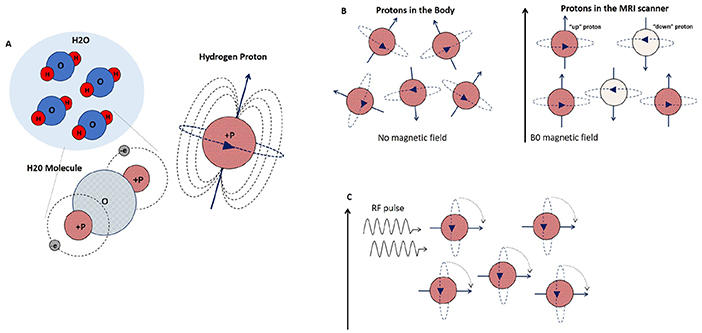
\includegraphics[width=80mm,scale=2]{tasos.jpg}
  \caption{Πρωτόνια υδρογώνου}
\end{figure*}
\begin{figure*}[h!]	
     \centering
     %\advance\leftskip-2.9cm  
  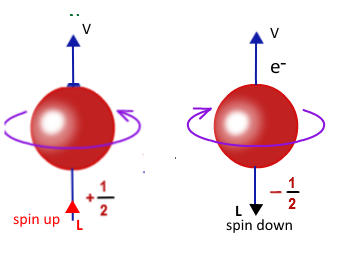
\includegraphics[width=80mm,scale=2]{spin.png}
  \caption{Περιστροφή πρωτονίων υδρογόνου}
\end{figure*}
\clearpage
\subsection{Μαγνητικός Συντονισμός}
Τα πρωτόνια του υδρογόνου μόλις τοποθετηθούν μέσα σε ενα πολύ ισχυρό μαγνήτη, διατάσσονται στο μαγνήτικο πεδίο, κάποια με περιστροφή προς τα πάνω και άλλα προς τα κάτω, συμπεριφερόμενα ως μαγνήτες που έχουν θετικούς και αρνητικούς πόλους. Κατα την λειτουργία του Μαγνητικού Τομογράφου εκπέμπονται μια σειρά δυνατών θορύβων που αντιπροσωπεύουν διαφορετικούς χειρισμούς των πρωτονίων. Στην πιο βασική του μορφή ο πρώτος θόρυβος αντιπροσωπεύει ένα ηλεκτρομαγνητικό πηνίο το οποίο ουσιαστικά είναι ένα κομμάτι κυκλικού χαλκού με ρεύμα που ρέει διαμέσου αυτού και είναι ενεργοποιημένο για ένα πολύ σύντομο χρονικό διάστημα. Συνήθως ανα λίγα χιλιοστά του δευτερολέπτου (ms) αυτό ωθεί ή περιστρέφει το πρωτόνιο από τον άξονά του εως 90 μοίρες, προκειμένου να έχουν όλα τα πρωτόνια ίδια διεύθυνση. Η συχνότητα του ηλεκτρομαγνητικού πηνίου, πρέπει να ταιριάζει ακριβώς με τη συχνότητα στην οποία τα πρωτόνια περιστρέφονται ή ό, τι καλούμε processing, είναι γνωστό ως η συντονισμένη ή η συχνότητα \textit{Larmor.}
\begin{figure*}[h!]	
     \centering
     %\advance\leftskip-2.9cm  
  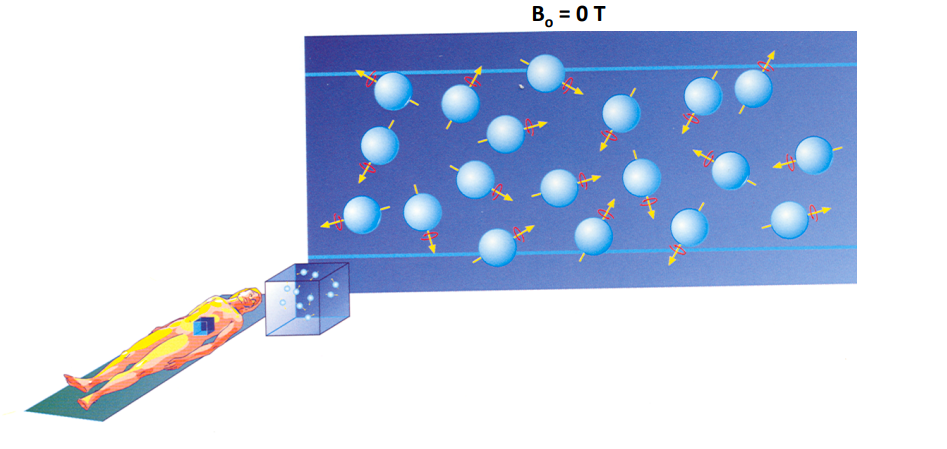
\includegraphics[width=80mm,scale=2]{mri0.png}
  \caption{Πρωτόνια υδρογώνου χωρίς την επίδραση εξωτερικου μαγνητικου πεδίου}
\end{figure*}

\begin{figure*}[h!]	
     \centering
     %\advance\leftskip-2.9cm  
  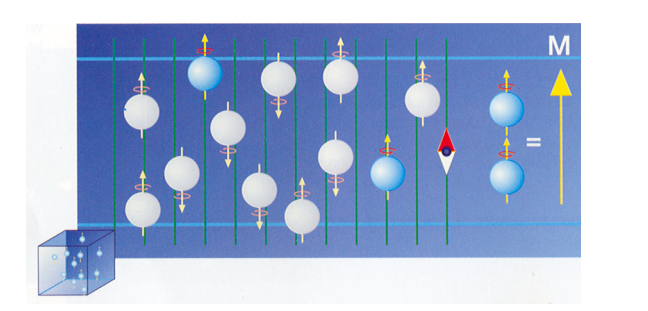
\includegraphics[width=75mm,scale=2]{mri1.png}
  \caption{Πρωτόνια υδρογώνου υπο την επίδραση ισχυρού εξωτερικου μαγνητικου πεδίου}
\end{figure*}

\clearpage
Όταν	 οι	 πυρήνες	 του	 υδρογόνου	 (πρωτόνια)	 εκτεθούν	 σε	
ισχυρό	 εξωτερικό	 μαγνητικό	 πεδίο,	 ευθυγραμμίζονται	
παράλληλα	(με	την	ίδια	φορά)	ή	αντιπαράλληλα	(με	αντίθετη	
φορά)	με	τον	άξονα	των	δυναμικών	γραμμών	του	εξωτερικού	
πεδίου. \\
\textit{Συχνότητα	Larmor: $ω_L$ = συχνότητα	
μεταπτωτικής	κίνησης	}
\begin{figure*}[h!]	
     \centering
     %\advance\leftskip-2.9cm  
  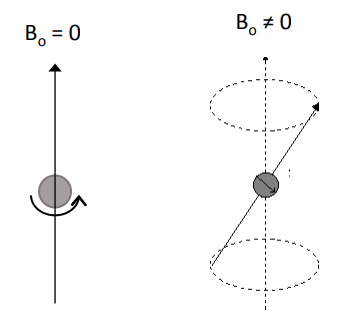
\includegraphics[width=80mm,scale=2]{ms.png}
  \caption{Αλληλεπίδραση υδρογώνου	με	εξωτερικό	μαγνητικό	πεδίο}
\end{figure*}

Για	τους	πυρήνες	υδρογόνου	:	
\begin{equation*}
    Β_0	=	0.5	Τ \implies ω_L = 21.3	ΜHz 
\end{equation*}
\begin{equation*}
    Β_0	=	1.5	Τ \implies ω_L = 42.6	ΜHz 
\end{equation*}
\begin{equation*}
    Β_0	=	3.0	Τ \implies ω_L = 127.7	ΜHz 
\end{equation*}
\begin{figure*}[h!]	
     \centering
     \advance\leftskip-0.8cm  
  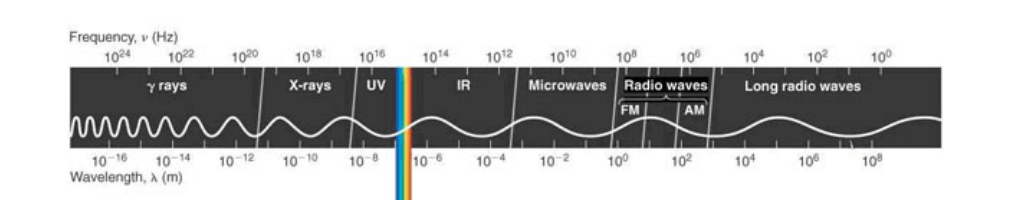
\includegraphics[width=140mm,scale=2]{msa.png}
 
\end{figure*}
\clearpage
\subsection{Συντονισμός	–	Διέγερση	πυρήνων}
Το	 άνυσμα	 Μ	 εκτελεί	 μετάπτωση.	 Με	 κατάλληλη	
επιλογή	της	έντασης	και	του	χρονικού	διαστήματος	
εφαρμογής	 του	 Β1,	 επιτυγχάνεται	 η	 επιθυμητή	
γωνία	νεύσης	φ (φ=γ$Β_1$t).	Στο	σχήμα	παρουσιάζεται	
η	 θέση	 του	 ανύσματος	 της	 ολικής	 μαγνήτισης,	Μ,	
μετά	την	εφαρμογή	παλμού	α)	$90^{ο}$	και	β)	$180^{ο}$.	


\begin{figure*}[h!]	
     \centering
     
  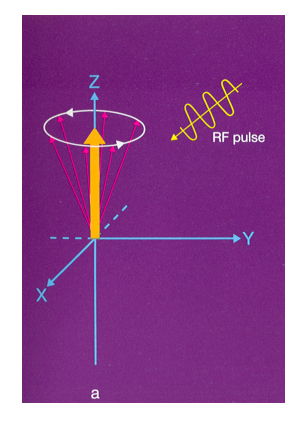
\includegraphics[width=50mm,scale=0.6]{t1.png}
  \caption{Συντονισμός	–	Διέγερση	πυρήνων}
\end{figure*}

\begin{figure*}[h!]	
     \centering
     
  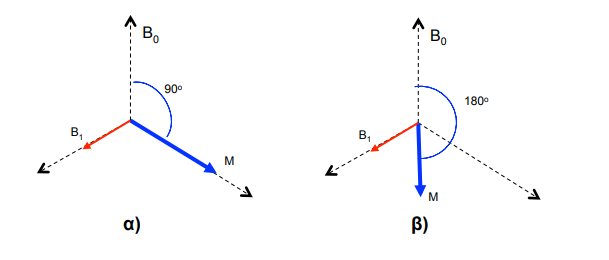
\includegraphics[width=120mm,scale=1.8]{t2.png}
  \caption{Συντονισμός	–	Διέγερση	πυρήνων}
\end{figure*}
\clearpage

\subsection{Μηχανισμοί	αποκατάστασης	–	αποδιέγερσης}
Μετά	 τη	 λήξη	 του	 ραδιοπαλμού	 $B_{1}\\
$,	 η	 μαγνήτιση	 Μ	 περιστρέφεται	
γύρω	από	το	στατικό	πεδίο	$Β_{ο}$	με	τη	συχνότητα	Larmor	και	σταδιακά	
επανέρχεται	από	τη	διεγερμένη	κατάσταση	(όπου	η	μαγνήτιση	είναι	
κάθετη	στο	$Β_{ο}$)	στην	αρχική	κατάσταση	θερμοδυναμικής	ισορροπίας	
(όπου	η	μαγνήτιση	είναι	παράλληλη	στο	$Β_{ο}$).
 Η	 επαναφορά	 αυτή	 πραγματοποιείται	 με	
δύο	 διαφορετικούς	 μηχανισμούς	 οι	 οποίοι	
έχουν	να	κάνουν
\begin{itemize}
    \item με	τη	αποκατάσταση	της	διαμήκους	
μαγνήτισης	$M_z$	η	οποία	αυξάνεται	με	το	
χρόνο
    \item την	αποκατάσταση	της	εγκάρσια	
μαγνήτισης	$Μ_{xy}$	η	οποία	μειώνεται	με	το	
χρόνο.		
\end{itemize}
\begin{figure*}[h!]	
     \centering
     
  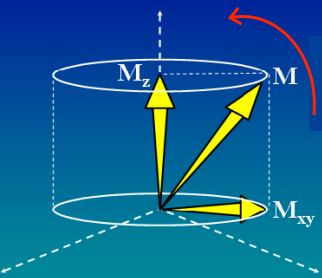
\includegraphics[width=100mm,scale=1.4]{mxy.png}
  \caption{Μηχανισμοί	αποκατάστασης	–	αποδιέγερσης}
\end{figure*}
\clearpage

\begin{itemize}
    \item \textbf{Σπιν	–	πλέγμα	 (spin - lattice relaxation)}.	Η	ενέργεια	που	προσφέρθηκε	
στο	 υπό	 εξέταση	 σύστημα	 πρωτονίων	 μεταφέρεται	 στο	 περιβάλλον	
του,	 το	 οποίο	 λόγω	 του	 μεγαλύτερου	 μεγέθους	 απορροφά	 την	
ενέργεια	 χωρίς	 να	 διεγείρεται.	 Με	 τον	 όρο	 πλέγμα	 εννοούμε	 το	
γειτονικό	 ηλεκτρομαγνητικό	 περιβάλλον	 του	 υπό	 εξέταση	 πυρηνικού	
συστήματος.		
\item\textbf{ Σπιν	–	Σπιν	(spin-spin relaxation)}. Μετά	την	εφαρμογή	του	ραδιοπαλμού
$90^0$	 και	 λόγω	 της	 απορρόφησης	 ενέργειας,	 το	 σύστημα	 των	 πυρήνων	
βρίσκεται	 σε	 μια	 κατάσταση	 χαμηλής	 εντροπίας	 (οι	 επιμέρους	
μαγνητικές	 ροπές	 βρίσκονται	 σε	 συμφωνία	φάσεων).	Στη	 συνέχεια	 τα	
σπιν	των	πυρήνων	αλληλεπιδρούν	 	και	ανταλλάσουν	ενέργεια	μεταξύ	
τους.	 Οι	 ανταλλαγές	 αυτές	 ενέργειας	 δεν	 οδηγούν	 σε	 μεταβολή	 της	
εσωτερικής	 ενέργειας	 του	 συστήματος	 αλλά	 σε	 μεταβολή	 της	
εσωτερικής	του	εντροπίας	(τα	σπιν	παύουν	να	είναι	σε	φάση)	
\end{itemize}
\subsubsection{Χρόνος	μαγνητικής	αποκατάστασης	$Τ_1$}
Η	τιμή	του	χρόνου	$Τ_1$	εξαρτάται	από:	
\begin{itemize}
    \item Είδος	ιστού	
    \item Θερμοκρασία
    \item Ένταση	μαγνητικού	πεδίου
\end{itemize}
\subsubsection{Χρόνος	μαγνητικής	αποκατάστασης	$Τ_2$}
Η	τιμή	του	χρόνου	$Τ_2$	εξαρτάται	από:	
\begin{itemize}
    \item Δομή	ιστού	(κινητικότητα	πρωτονίων)	
    \item Θερμοκρασία	
    
\end{itemize}
\clearpage

\subsection{Σήμα	ελεύθερης	επαγωγικής	απόσβεσης}
Έστω	δείγμα	πρωτονίων	 το	οποίο	βρίσκεται	σε	ομογενές	μαγνητικό	πεδίο	$Β_o$	και	έχει	διεγερθεί	από	έναν	παλμό	$90^{o}$.
Μετά	 τη	 λήξη	 του	 παλμού,	 στο	 σταθερό	 σύστημα	 αναφοράς,	 το	 άνυσμα	
της	εγκάρσιας	μαγνήτισης	$M_{xy}$	εκτελεί	περιστροφική	κίνηση	στο	επίπεδο-xy
με	 κυκλική	 συχνότητα	 Larmor	 $ω_L$	 και	 το	 μέτρο	 του	 μειώνεται	 εκθετικά	
σύμφωνα	με	την	εξίσωση	
\begin{equation*}
    M_{xy}(t) =   M_{xy}(0) \cdot e^{-\frac{t}{T_2}}
\end{equation*}
   
    Τοποθετώντας	 ένα	 σωληνοειδές	 πηνίο	 το	 οποίο	 έχει	 τον	 κύριο	 άξονα	 του	
παράλληλο	 στο	 επίπεδο-xy,	 	 σύμφωνα	 με	 τον	 νόμο	 του	 Faraday,	 επάγεται	
τάση	στα	άκρα	 του	που	προέρχεται	από	 τις	μεταβολές	 της	μαγνητικής	 ροής,	
στις	σπείρες	του	πηνίου,	λόγω	της	περιστροφής	του	$M_{xy}$.

Η	 τάση	 αυτή	 είναι	 ένα	 διαμορφωμένο	 κατά	 πλάτος	 ηλεκτρικό	 σήμα	 με	
φέρουσα	συχνότητα	τη	συχνότητα	Larmor	$ω_L$	το	οποίο	μειώνεται	με	εκθετικό	
τρόπο	με	χρονική	σταθερά	τον	χρόνο	$Τ_2$	και	το	οποίο	παράγεται	αμέσως	μετά	
την	εφαρμογή	του	ραδιοπαλμού	$90^{ο}$.	
\subsection{Χωρική	πληροφορία	–	κωδικοποίηση	στο	χώρο	}
Στην	Απεικόνιση	Μαγνητικού	Συντονισμού	(ΑΜΣ)	όμως,	όπως	και	
σε	 όλες	 τις	 απεικονιστικές	 τεχνικές,	 απαιτείται	 η	 παραγωγή	
εικόνας	 με	 χωρική	 πληροφορία,	 με	 πληροφορία	 δηλαδή	 της	
θέσης	του	πυρήνα	που	διεγείρεται	ή	με	άλλα	λόγια	απαιτείται	η	
κωδικοποίηση	του	σήματος	στο	χώρο.	\\
Για	να	συμβεί	αυτό	πρέπει	το	μαγνητικό	πεδίο	να	μεταβάλλεται	
χωρικά	 έτσι	 ώστε	 να	 μεταβάλλεται	 χωρικά	 και	 η	 συχνότητα	
περιστροφής	 των	πυρήνων	 (συχνότητα	Larmor).	Στην	περίπτωση	
αυτή	οι	πυρήνες	μπορούν	να	διεγερθούν	επιλεκτικά	ανάλογα	με	
τη	θέση	τους	και	το	σήμα	που	θα	καταγραφεί	μπορεί	να	έχει	την	
χωρική	 πληροφορία	 που	 απαιτείται	 για	 την	 παραγωγή	 της	
εικόνας \\
Για	 το	 σκοπό	 αυτό,	 παράλληλα	 με	 το	 ισχυρό	
στατικό	 μαγνητικό	 πεδίο	 Βο	 εφαρμόζονται	
επιπλέον	 βαθμιδωτά	 πεδία	 η	 ένταση	 των	
οποίων	 μεταβάλλεται	 γραμμικά	 κατά	 μήκος	
του	άξονα	εφαρμογής	τους.	\\
H	 εφαρμογή	 των	 βαθμιδωτών	 πεδίων	
έχει	 ως	 αποτέλεσμα	 την	 χωρική	
βάθμωση	 των	 συχνοτήτων	 Larmor,	
δηλαδή	με	άλλα	λόγια	σε	κάθε	σημείο	
στον	 χώρο	 να	 αντιστοιχεί	 διαφορετική	
συχνότητα	Larmor.	\\
Διεγείροντας	 επιλεκτικά	 πυρήνες	 σε	 συγκεκριμένες	 χωρικές	 περιοχές	
και	εφαρμόζοντας	κατάλληλους	μετασχηματισμούς	Fourier	προκύπτουν	
εικόνες	 με	 χωρική	 πληροφορία,	 οι	 οποίες	 αντιστοιχούν	 σε	 τομές	 του	
σώματος.	\\
Οι	εικόνες	αυτές	αναπαριστούν	τα	μαγνητικά	χαρακτηριστικά	του	ιστού	
που	απεικονίζεται	στην	κάθε	περιοχή-τομή	και	αποτελούνται	από	έναν	
πίνακα	 εικονοστοιχείων	 (pixels)	 όπου	 η	 φωτεινότητα	 (brightness)	 του	
καθενός	 σχετίζεται	 με	 τις	 μαγνητικές	 ιδιότητες	 του	 αντίστοιχου	
ογκοστοιχείου	(voxel).	 \\
Το	 σήμα	 από	 κάθε	 voxel	 είναι	 η	 μέση	 τιμή	 των	 σημάτων	 όλων	 των	
πρωτονίων	που	περιέχει.	\\
Ενεργοποιώντας	το	πηνίο	βάθμωσης	στον	άξονα-z	 (z-gradient)	
τα	πρωτόνια	κατά	μήκος	του	άξονα	“αισθάνονται”	διαφορετικό	
πεδίο	 και	 αποκτούν	 γραμμικά	 μεταβαλλόμενες	 συχνότητες	
Larmor.	\\
Τα	 πρωτόνια	 της	 τομής	 που	 μας	 ενδιαφέρει	 έχουν	 ένα	
μοναδικό	φάσμα	συχνοτήτων	το	οποίο	μας	είναι	γνωστό.	 \\
Αν	εκπεμφθεί	ένας	παλμός	900	ειδικά	διαμορφωμένος	ώστε	να	
περιέχει	 τις	 συχνότητες	 των	 πρωτονίων	 της	 τομής	 	 τότε	
διεγείρονται	 μόνο	 τα	 πρωτόνια	 της	 τομής.	 Η	 κεντρική	
συχνότητα	 του	 παλμού	 καθορίζει	 το	 ύψος	 της	 τομής	 ενώ	 το	
εύρος	ζώνης	συχνοτήτων	(bandwidth)	καθορίζει	το	πάχος	της.		\\
\begin{figure*}[h!]	
     \centering
     %\advance\leftskip-2.9cm  
  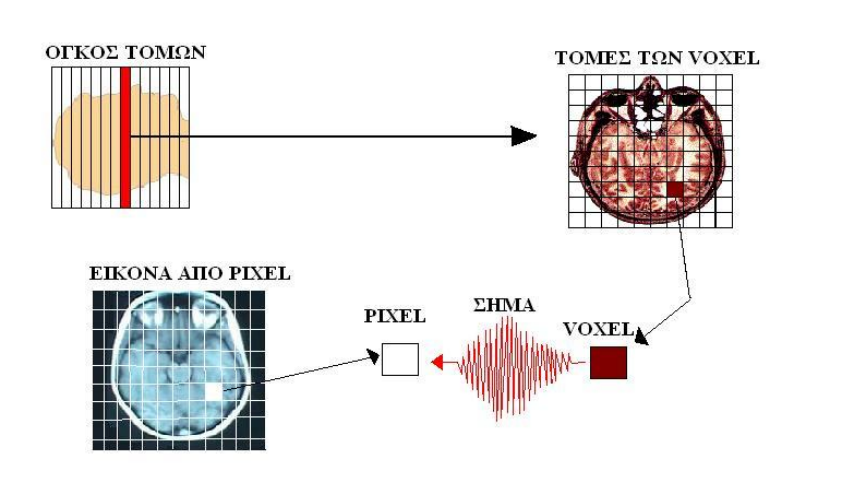
\includegraphics[width=80mm,scale=2]{end.png}
  \caption{Χωρική	πληροφορία	–	κωδικοποίηση	στο	χώρο}
\end{figure*}
\clearpage











\section{Ιστορική Εξέλιξη}
\subsection{Αρχικές Έρευνες}
Αρχικά το 1924 ο Pauli πρότεινε την θεωρητική
ύπαρξη μιας εγγενούς πυρηνικής περιστροφής. Το 1925 οι Uhlenbeck και Goudsmit
εισήγαγαν στην φυσική την έννοια του περιστρεφόμενου ηλεκτρονίου. Δύο χρόνια αργότερα,
ο Pauli και ο Charles Galton Darwin ανέπτυξαν ένα θεωρητικό πλαίσιο για την έννοια της
περιστροφής ηλεκτρονίων με βάση τους νόμους της κβαντικής μηχανικής που αναπτύχθηκαν
από τον Έρβιν Σρέντινγκερ και τον Βέρνερ Χάιζενμπεργκ.
Οι πρώτες μελέτες σχετικά με τις μαγνητικές ιδιότητες των πυρήνων ξεκινούν στις
αρχές της δεκαετίας του '30 με τους Gorter και Rabi. Το 1933 o Otto Stern και o Walther
Gerlach ήταν σε θέση να μετρήσουν την επίδραση της πυρηνικής περιστροφής από την
εκτροπή μιας ακτίνας μορίων υδρογόνου. Κατά τη διάρκεια της δεκαετίας του '30, το
εργαστήριο του Isidor Isaac Rabi στο πανεπιστήμιο Κολούμπια της Νέας Υόρκης έγινε
σημαντικό κέντρο σχετικών μελετών.
\subsection{H φασματοσκοπία (NMR)}
Ο Gorter χρησιμοποίησε αρχικά τον όρο "πυρηνικός
μαγνητικός συντονισμός" σε μια δημοσίευση που εμφανίστηκε στην Ολλανδία το 1942.
Ο μαγνητικός συντονισμός περιστροφής ηλεκτρονίων ανακαλύφθηκε στο
πανεπιστήμιο Κazan από τον Yevgeni Κ. Zavoisky προς το τέλος του 1943. Ο Zavoisky είχε
ανιχνεύσει τον πυρηνικό μαγνητικό συντονισμό το 1941 και παρουσίασε τα πορίσματά του
σε αγγλόφωνο ρωσικό επιστημονικό περιοδικό, αλλά δεν είχε αντίκτυπο στην επιστημονική
κοινότητα της εποχής. Επίσημα το φαινόμενο του πυρηνικού μαγνητικού συντονισμού
(nuclear magnetic resonance-NMR) ανακαλύφθηκε ανεξάρτητα από τους Φέλιξ Μπλοχ
(Stanford) και Έντουαρντ Πάρσελ (Harvard) το 1946 και το 1952 βραβεύονται με βραβείο
Νόμπελ φυσικής.
4
Λίγα χρόνια αργότερα αναπτύχθηκε η φασματοσκοπία NMR, η οποία ξεκινά να
εφαρμόζεται κυρίως για την in vitro έρευνα στοιχείων και χημικών ενώσεων (σε μελέτες με
πολλές τεχνικές δυσκολίες και με αρκετά σφάλματα). Το 1955/1956, ο Erik Odeblad και ο
Gunnar Lindstrοm από τη Στοκχόλμη δημοσίευσαν τις πρώτες μελέτες ΝΜR,
συμπεριλαμβανομένων μετρήσεων χρόνων χαλάρωσης, μελετών ζωντανών κυττάρων και
αξιολόγησης ζωικών ιστών. Ο Odeblad συνέχισε τις μελέτες σε ζωντανούς ιστούς καθ' όλη τη
διάρκεια της δεκαετίας του '50 και του '60. Το 1959 o Jay Singer μελέτησε την δυνατότητα
μέτρησης ροών σε ιστούς. Στα τέλη της δεκαετίας του '60 γίνονται έρευνες για την λήψη
σημάτων και προσδιορισμού των χρόνων χαλάρωσης σε ανθρώπους και σε ζώα με κυριότερη
την μελέτη του J. Johns, ο οποίος μελέτησε την χημική σύσταση των ιστών ζωντανών ζώων
(1967). 
\subsection{Η συμβολή του αξονικού τομογράφου}
Η εφεύρεση του αξονικού τομογράφου στα μέσα της δεκαετίας του '60 επηρέασε
θετικά την έρευνα για την εξέλιξη των εφαρμογών απεικόνισης μαγνητικού συντονισμού.
Μερικές εβδομάδες μετά την εγκατάσταση του πρώτου αξονικού τομογράφου (Αγγλία, 1971)
ο Paul Lauterbur ανακαλύπτει την δυνατότητα χωρικής χαρτογράφησης των μοριακών
συγκεντρώσεων συνδυάζοντας τα γραμμικά βαθμιδωτά πεδία (χρησιμοποιήθηκαν πρώτη
φορά από τον Erwin L.Hahn το 1950) και την τεχνική της οπισθοπροβολής (σε αυτή
βασίζεται η αξονική τομογραφία).
\subsection{H φασματοσκοπία φωσφόρου}
Στις αρχές της δεκαετίας του 1970 πραγματοποιούνται οι πρώτες μελέτες της
φασματοσκοπίας φωσφόρου για την ανάλυση δειγμάτων ερυθροκυττάρων (Moon 1973). Το
1974 ο Hoult μελετά με την φασματοσκοπία φωσφόρου την σύσταση των μυικών ιστών
ποντικών. Τότε γίνεται φανερό ότι η φασματοσκοπία προσφέρει μη επεμβατική in vivo
ανάλυση της σύστασης και του μεταβολισμού των ιστών.
Το 1972 ο Raymond Damadian ανακαλύπτει ότι οι παθολογικοί ιστοί εμφανίζουν
μεγαλύτερους χρόνους χαλάρωσης σε σχέση με τους αντίστοιχους υγιείς. Το 1973 ο
Lauterbur παρουσιάζει την εικόνα δυο σωλήνων με νερό στο περιοδικό Nature και το 1974
παρουσιάζει την απεικόνιση της θωρακικής κοιλότητας ενός ποντικού. Ονόμασε την τεχνική
αυτή ζευγματογραφία, όρος ο οποίος μετέπειτα αντικαταστάθηκε από τον όρο απεικόνιση
μαγνητικού συντονισμού. Το 1974 οι Anil Kumar, Dieter Welti και Richard Ernst
παρουσίασαν την εργασία 'NMR Fourier Zeugmatography' η οποία περιγράφει την χρήση
χρονικά μεταβαλλόμενων βαθμιδωτών πεδίων και την εφαρμογή των μετασχηματισμών
Fourier για την ανακατασκευή των εικόνων. Επίσης το 1974 η εταιρία ΕΜΙ ασχολήθηκε με
την κατασκευή εξοπλισμού αυτού του είδους. Με την συνεισφορά και των εργασιών του
Damadian και τις ανακαλύψεις του Lauterbur επήλθε επανάσταση στην ιατρική απεικόνιση
καθώς οδήγησε στην δημιουργία του πρώτου υποτυπώδους πειραματικού μαγνητικού
τομογράφου.
5
\subsection{Ο πρώτος μαγνητικός τομογράφος}
Οι καθηγητές Damadian, Minkoff και Goldsmith, μόλις ολοκλήρωσαν την
κατασκευή του πρώτου υποτυπώδους μαγνητικού τομογράφου (Indomitable), στις 3 Ιουλίου
1977, μετά από μέτρηση 6 ωρών και ανακατασκευή 22 ωρών παρήγαγαν την πρώτη ιατρική
εικόνα του ανθρώπινου σώματος (τομή θωρακικής χώρας).
Επίσης το 1977 ο Sir Peter Mansfield και η ομάδα του έλαβαν εικόνες από τομή
δακτύλου του χεριού και από την κοιλιακή χώρα με την βοήθεια της τεχνικής Echo Planar
Imaging (E.P.I.).
\subsection{Διαθεσιμότητα του μαγνητικου τομογράφου στο εμπόριο}
Το 1992 εμφανίστηκε ο πρώτος εμπορικά διαθέσιμος μαγνητικός τομογράφος για
ιατρικές εφαρμογές. Στις μέρες μας υπάρχουν περίπου 30000 μαγνητικοί τομογράφοι σε
λειτουργία για ιατρική χρήση σε παγκόσμιο επίπεδο, ενώ παρασκευάζονται 2000 καινούργιοι
κάθε χρόνο. Οι Ηνωμένες Πολιτείες Αμερικής αντιπροσωπεύουν το 40\% της παραγωγής των
μαγνητικοών τομογράφων. 

\end{document}
